\documentclass[10pt]{article}
\usepackage[spanish]{babel}
\usepackage[a4paper, tmargin=0.75in, lmargin=0.80in, rmargin=0.80in, bmargin=1in]{geometry}
\usepackage{hyperref}
%\usepackage{multicol}
\hypersetup{
    colorlinks=true,
    linkcolor=black,
    filecolor=magenta,      
    urlcolor=blue,
    citecolor=black,
}
%\usepackage[numbers,sort&compress]{natbib} % for a numerical citation list
\usepackage{natbib} % to cite references by surname and year
\usepackage{graphicx}
\usepackage{amsfonts}
\usepackage{amsthm}
\usepackage{amssymb}
\usepackage{lipsum}
\usepackage{amsmath}
\usepackage{tabularx}
\usepackage{pdflscape}
\usepackage{booktabs}
\usepackage{bbm}
\usepackage{listings}
\usepackage{xcolor}

\usepackage[
  backend=biber,
  style=alphabetic,
  citestyle=alphabetic,
  doi=true,
  url=true,
  isbn=false,
  eprint=false,
  maxbibnames=99
]{biblatex}

\addbibresource{referencias.bib}

% Definimos colores estilo "terminal con fondo negro"
\definecolor{backcolour}{rgb}{0.1,0.1,0.1}
\definecolor{codegreen}{rgb}{0,0.8,0}
\definecolor{codegray}{rgb}{0.7,0.7,0.7}
\definecolor{codepurple}{rgb}{0.8,0.6,1}
\definecolor{codewhite}{rgb}{1,1,1}


\lstdefinestyle{mypython}{
    backgroundcolor=\color{backcolour},
    basicstyle=\ttfamily\scriptsize\color{codewhite},
    commentstyle=\color{codegreen},
    keywordstyle=\color{codepurple},
    stringstyle=\color{codegreen},
    numbers=left,
    numberstyle=\tiny\color{codegray},
    breaklines=true,
    breakatwhitespace=false,
    showstringspaces=false,
    tabsize=4
}

\lstset{style=mypython}







\pagestyle{empty}


%%%%%%%%%%%%%%%%%%%%%%%%%%%%%%%%%%%%%%%%%%%%%%%%%%
%%%%%%%%%%%%%%%%%%%%%%%%%%%%%%%%%%%%%%%%%%%%%%%%%%
%%%%%%%%%%%%%%%%%%%%%%%%%%%%%%%%%%%%%%%%%%%%%%%%%%
%%%%%%%%%%%%%%%%%%%%%%%%%%%%%%%%%%%%%%%%%%%%%%%%%%
% ENTER SOME IMPORTANT INFORMATION
%%%%%%%%%%%%%%%%%%%%%%%%%%%%%%%%%%%%%%%%%%%%%%%%%%
%%%%%%%%%%%%%%%%%%%%%%%%%%%%%%%%%%%%%%%%%%%%%%%%%%
%%%%%%%%%%%%%%%%%%%%%%%%%%%%%%%%%%%%%%%%%%%%%%%%%%
%%%%%%%%%%%%%%%%%%%%%%%%%%%%%%%%%%%%%%%%%%%%%%%%%%
\newcommand{\studentname}{Sánchez, Hazel; Hernández, Debany ; Canché, Elías}
\newcommand{\researchcentre}{Maestría en Probabilidad y Estadística}
\newcommand{\institution}{Centro de Investigación en Matemáticas (CIMAT)}
\newcommand{\projecttitle}{Tarea 2}
\newcommand{\supervisor}{Dr. Marco Antonio Aquino López}
%%%%%%%%%%%%%%%%%%%%%%%%%%%%%%%%%%%%%%%%%%%%%%%%%%
%%%%%%%%%%%%%%%%%%%%%%%%%%%%%%%%%%%%%%%%%%%%%%%%%%
%%%%%%%%%%%%%%%%%%%%%%%%%%%%%%%%%%%%%%%%%%%%%%%%%%
%%%%%%%%%%%%%%%%%%%%%%%%%%%%%%%%%%%%%%%%%%%%%%%%%%
%%%%%%%%%%%%%%%%%%%%%%%%%%%%%%%%%%%%%%%%%%%%%%%%%%
%%%%%%%%%%%%%%%%%%%%%%%%%%%%%%%%%%%%%%%%%%%%%%%%%%

\begin{document}

\begin{center}
{\Large{Proyecto 2: Clasificación Supervisada}} \\
\vspace{2mm}
{\Large{Introducción a la Ciencia de Datos}} \\
\end{center}

\vspace{5mm}
\hrule
\vspace{1mm}
\hrule

\vspace{3mm}
\begin{tabular}{ll} 
Integrantes:           	        & {\studentname}   \\ 
Programa Educativo: 	        & {\researchcentre}  \\ 
Institución:                 & {\institution}  \\
Profesor: 	                 & {\supervisor}  \\ 
\end{tabular}

\vspace{3mm}
\hrule
\vspace{1mm}
\hrule

\begin{abstract}

\end{abstract}
\section{Análisis computacional mediante simulaciones (Segunda Parte de la Tarea)}

\subsection*{Introducción}

El propósito de esta segunda parte es estudiar, en un entorno controlado donde
la distribución verdadera de las clases son conocidas, el comportamiento de los
clasificadores vistos en el curso frente al clasificador óptimo (de Bayes).

Para este propósito, se diseñan y ejecutan simulaciones con datos sintéticos
generados a partir de distribuciones normales multivariadas (en dos
dimensiones), comparamos el riesgo de clasificación de cada método tanto contra
el riesgo óptimo como contra estimadores obtenidos por métodos de validación, 
para estas comparaciones variamos parámetros como los tamaños de muestras y
valores de $k$ (en \textit{k-NN}). Además, para simplifcar el calculo del error
de Bayes teórico y comporarlo con los otros errores, se utilizan muestras
proporcionales y con covarianzas iguales para las dos clases.



\subsection*{Comportamiento de clasificadores}

A continuación se muestran los resultados obtenidos en las simulaciones
realizadas. Consideramos los siguientes casos para cada simulación:

\begin{itemize}
    \item \texttt{Clases separadas}: Mismas covarianzas para ambas clases.
    \item \texttt{Clases sobrepuestas}: Distintas covarianzas para ambas clases.
    \item \texttt{Datos balanceados}: Mismos tamaños de muestras para ambas
    clases.
    \begin{itemize}
        \item Mismas covarianzas
        \item Distintas covarianzas
    \end{itemize}
    \item \texttt{Datos desbalanceados}: Tamaños de muestras distintos
    (proporciones de 0.2 y 0.8).
    \begin{itemize}
        \item Mismas covarianzas
        \item Distintas covarianzas
    \end{itemize}
\end{itemize}


\subsubsection*{Clases separadas}

Los clasificadores con las clases separadas se comportaron como la Figura
\ref{fig:classifier-comparison-balanced-separated-classes}.
\begin{figure}[!ht]
    \centering
    \includegraphics[height=0.4\textheight]{./Parte 2/figures/classifier_comparison_balanced_separated_classes.png}
    \caption{Comportamiento de clasificadores con datos balanceados y clases separadas.}    
    \label{fig:classifier-comparison-balanced-separated-classes}
\end{figure}

% Argumentar lo de arriba
\newpage

\subsubsection*{Clases sobrepuestas}

Los clasificadores con las clases sobrepuestas se comportaron como la Figura
\ref{fig:classifier-comparison-balanced-joined-classes}.

\begin{figure}[!ht]
    \centering
    \includegraphics[height=0.4\textheight]{./Parte 2/figures/classifier_comparison_balanced_joined_classes.png}
    \caption{Comportamiento de clasificadores con datos balanceados y clases separadas.}    
    \label{fig:classifier-comparison-balanced-joined-classes}
\end{figure}

% Argumentar lo de arriba
\newpage

\subsubsection*{Datos Balanceados}

A partir de este punto, las simulaciones se realizan con las medias
$\mu_0=(-1,0)$ y $\mu_1=(0, 1)$ para sus respectivas clases, a menos que se
indique lo contrario.

Para datos generados con la misma covarianza se observan las siguientes
comparaciones en la Figura \ref{fig:classifier-comparison-balanced-same-cov}

\begin{figure}[!ht]
    \centering
    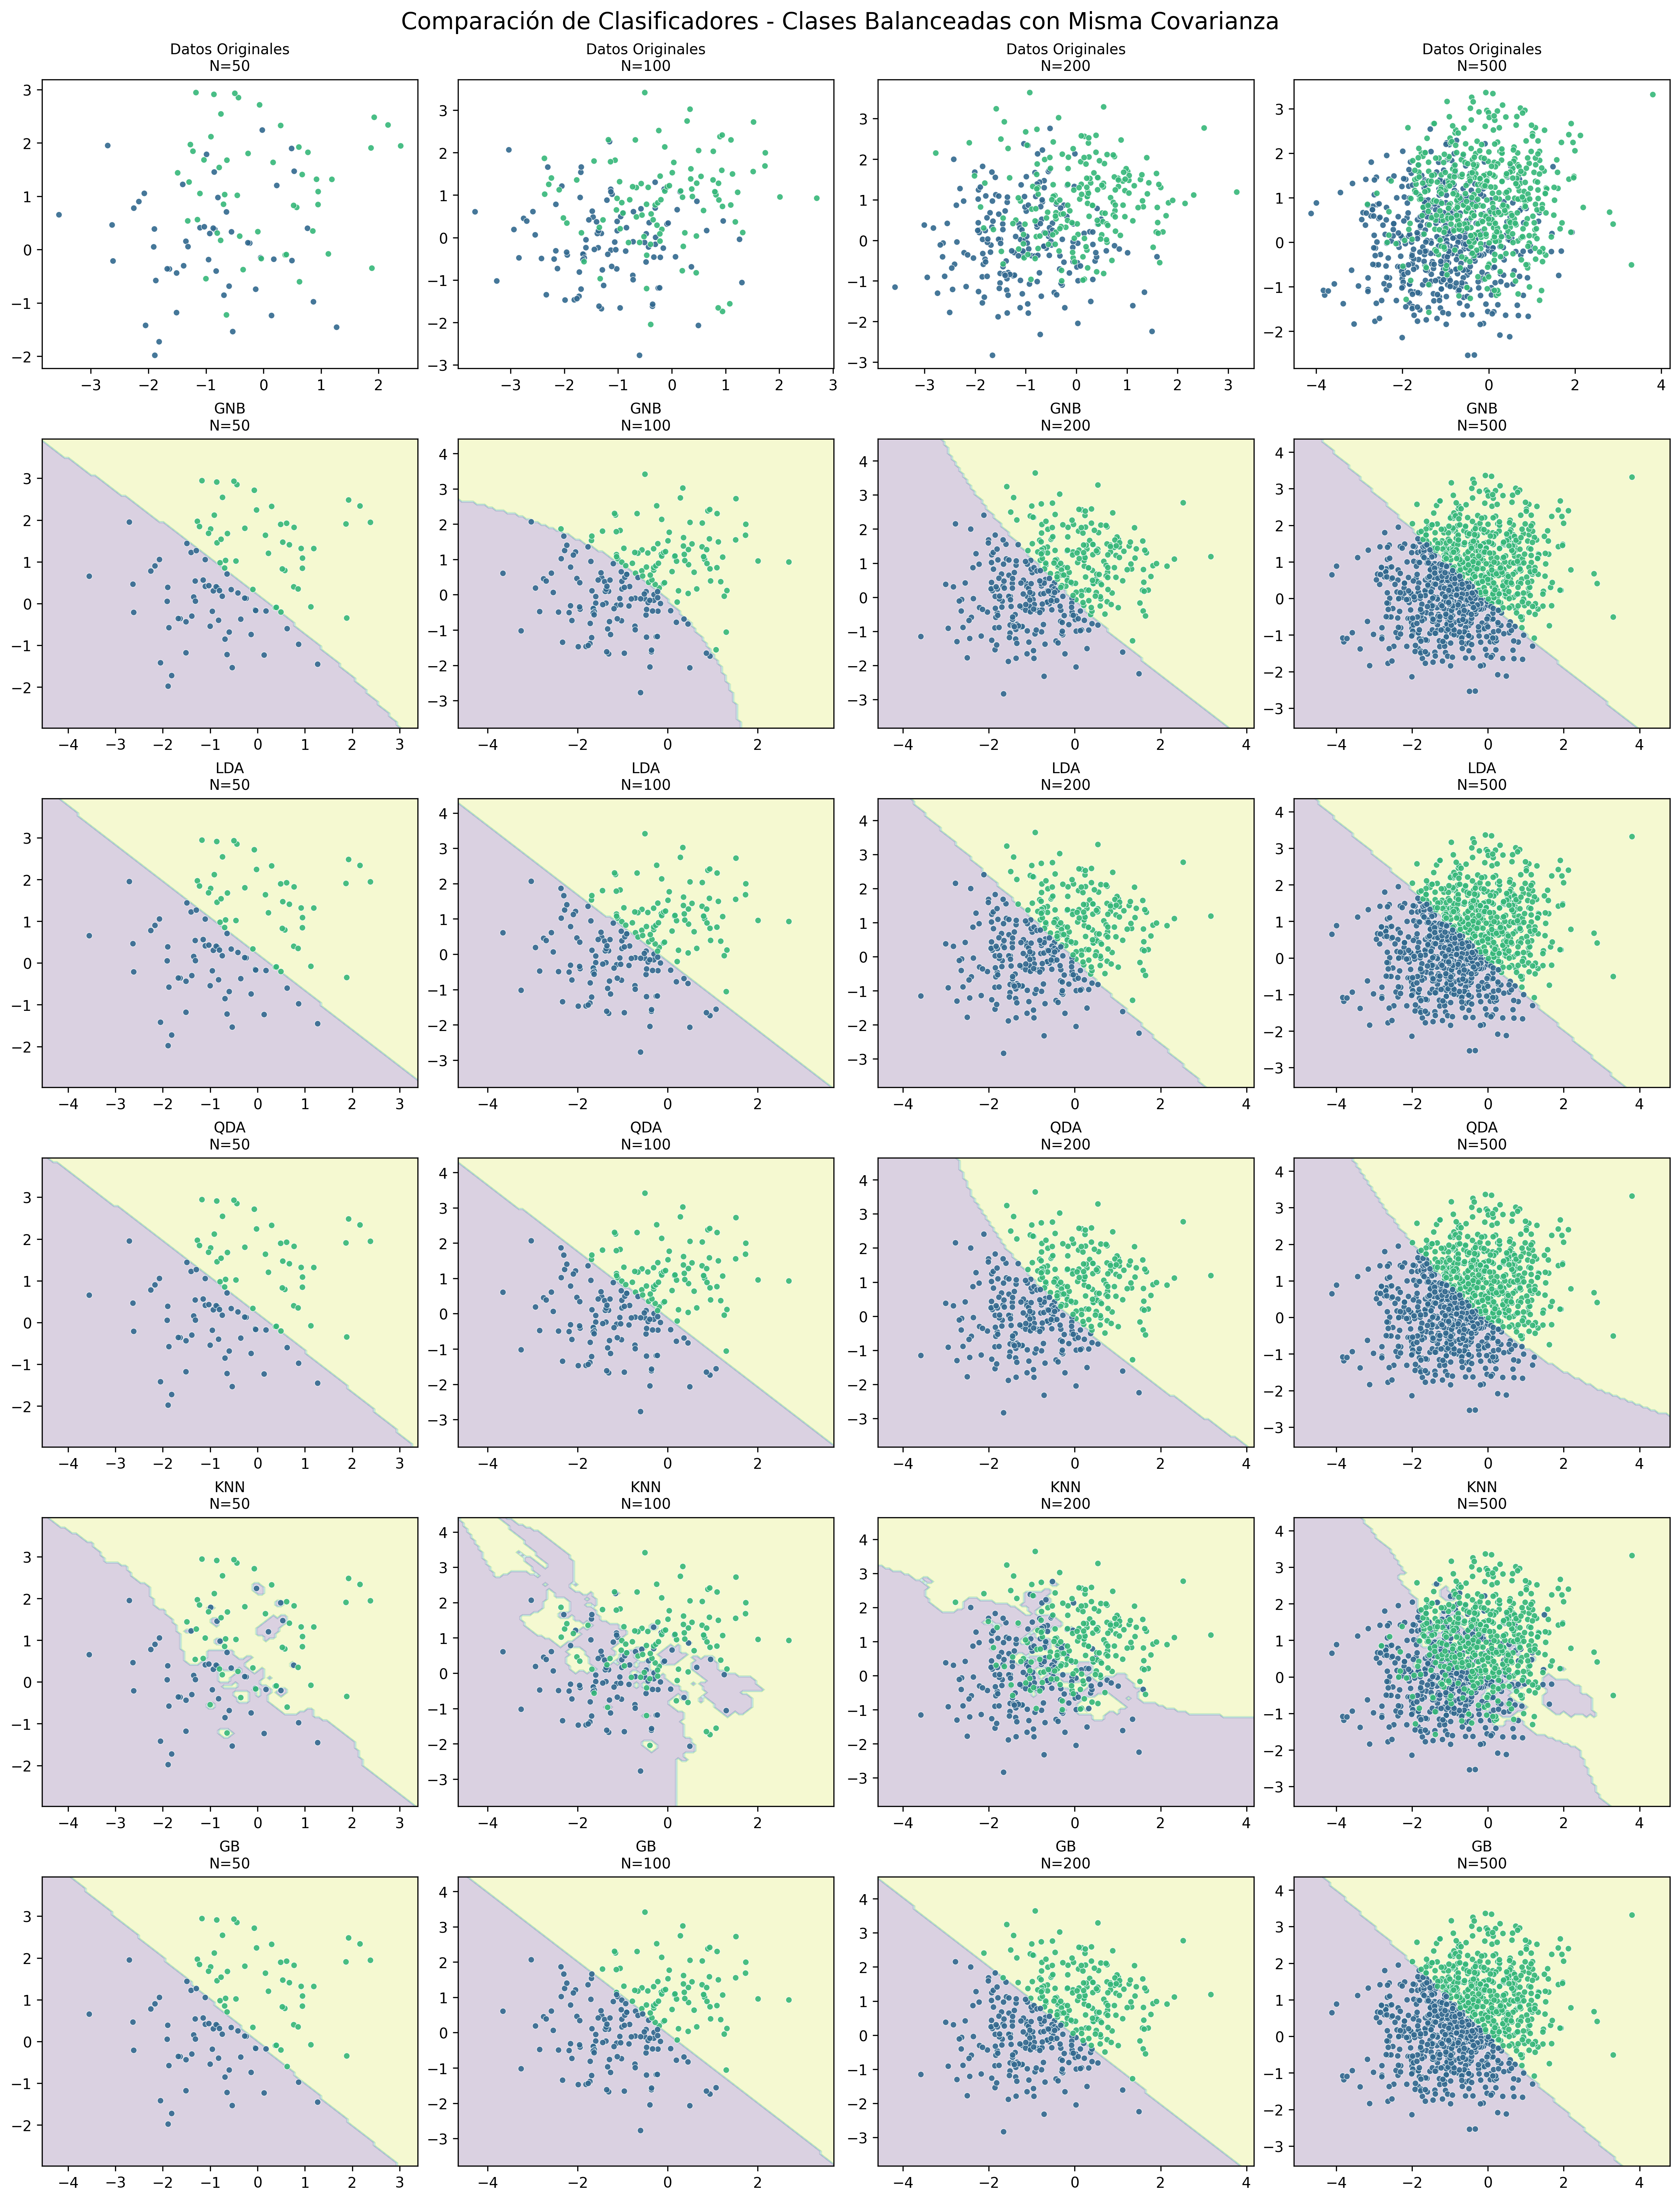
\includegraphics[height=0.4\textheight]{./Parte 2/figures/classifier_comparison_balanced_same_cov.png}
    \caption{Comportamiento de clasificadores con datos balanceados y covarianzas iguales.}    
    \label{fig:classifier-comparison-balanced-same-cov}
\end{figure}

\newpage

Para datos generados con distintas covarianzas se observan las siguientes
comparaciones en la Figura \ref{fig:classifier-comparison-balanced-distinct-cov}

\begin{figure}[!ht]
    \centering
    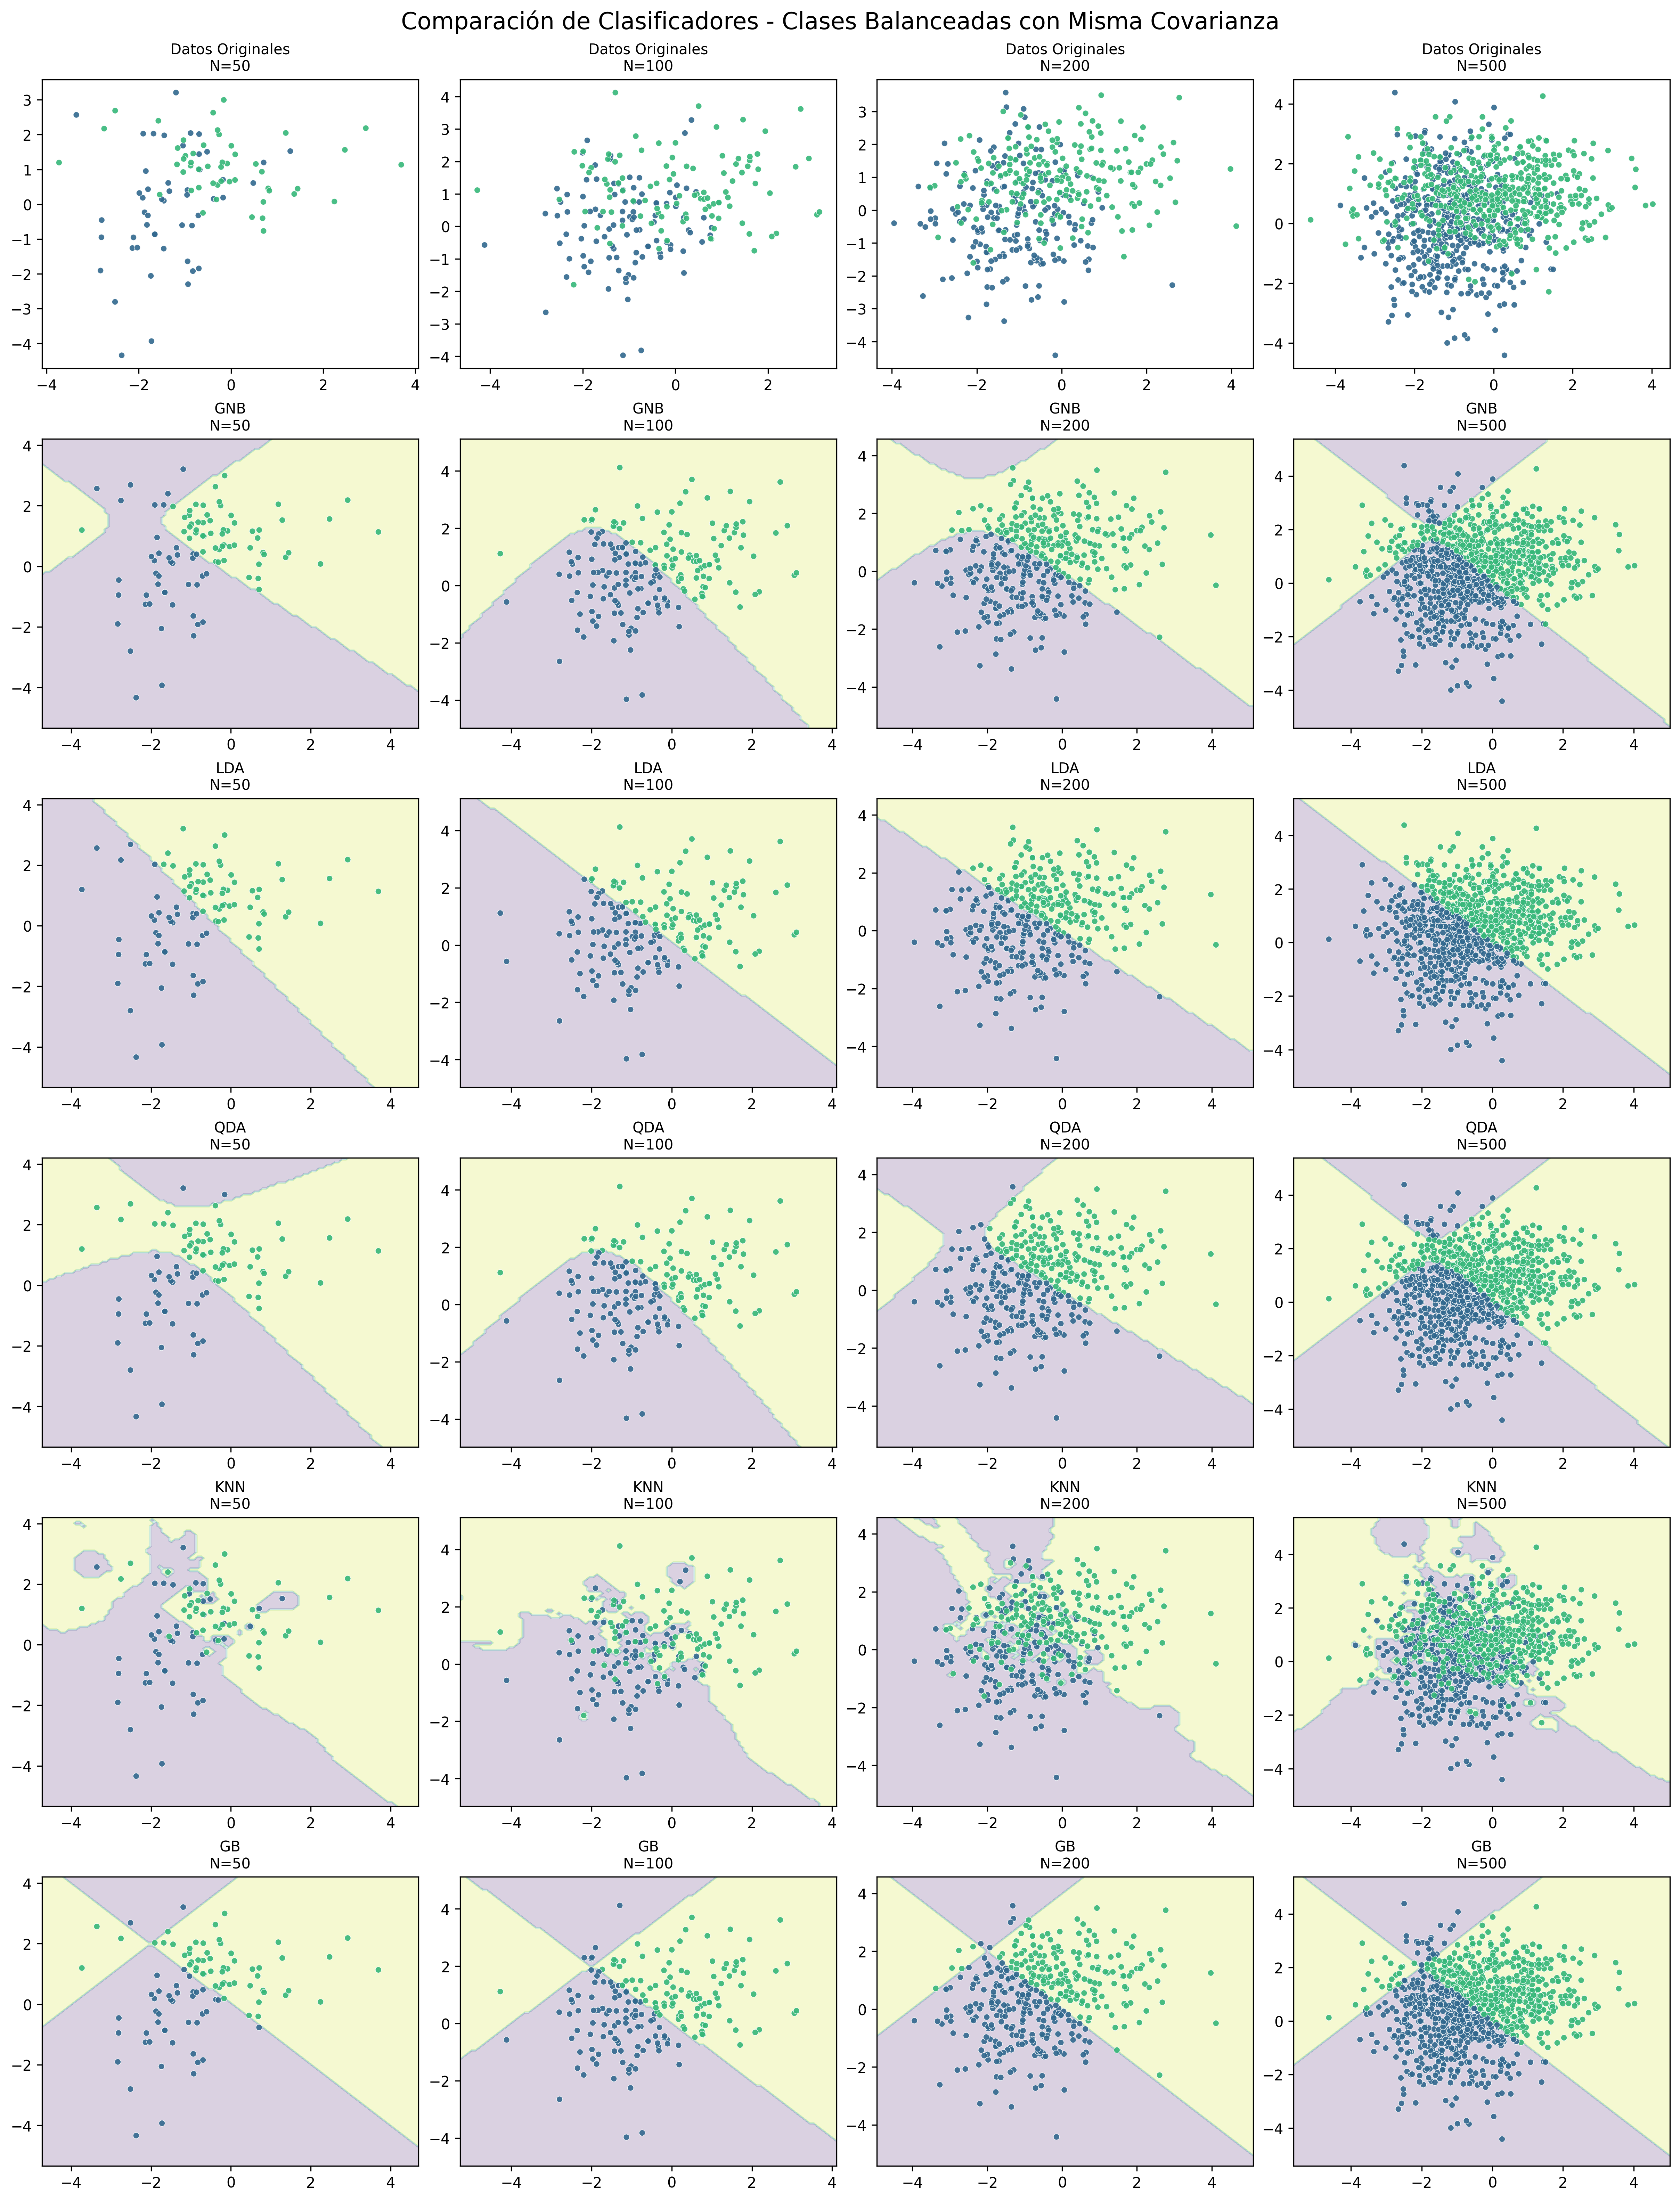
\includegraphics[height=0.4\textheight]{./Parte 2/figures/classifier_comparison_balanced_distinct_cov.png}
    \caption{Comportamiento de clasificadores con datos balanceados y covarianzas distintas.}    
    \label{fig:classifier-comparison-balanced-distinct-cov}
\end{figure}

% Argumentar lo de arriba
\newpage

\subsubsection*{Datos Desbalanceados}

Para datos generados con la misma covarianza se observan las siguientes
comparaciones en la Figura \ref{fig:classifier-comparison-unbalanced-same-cov}

\begin{figure}[!ht]
    \centering
    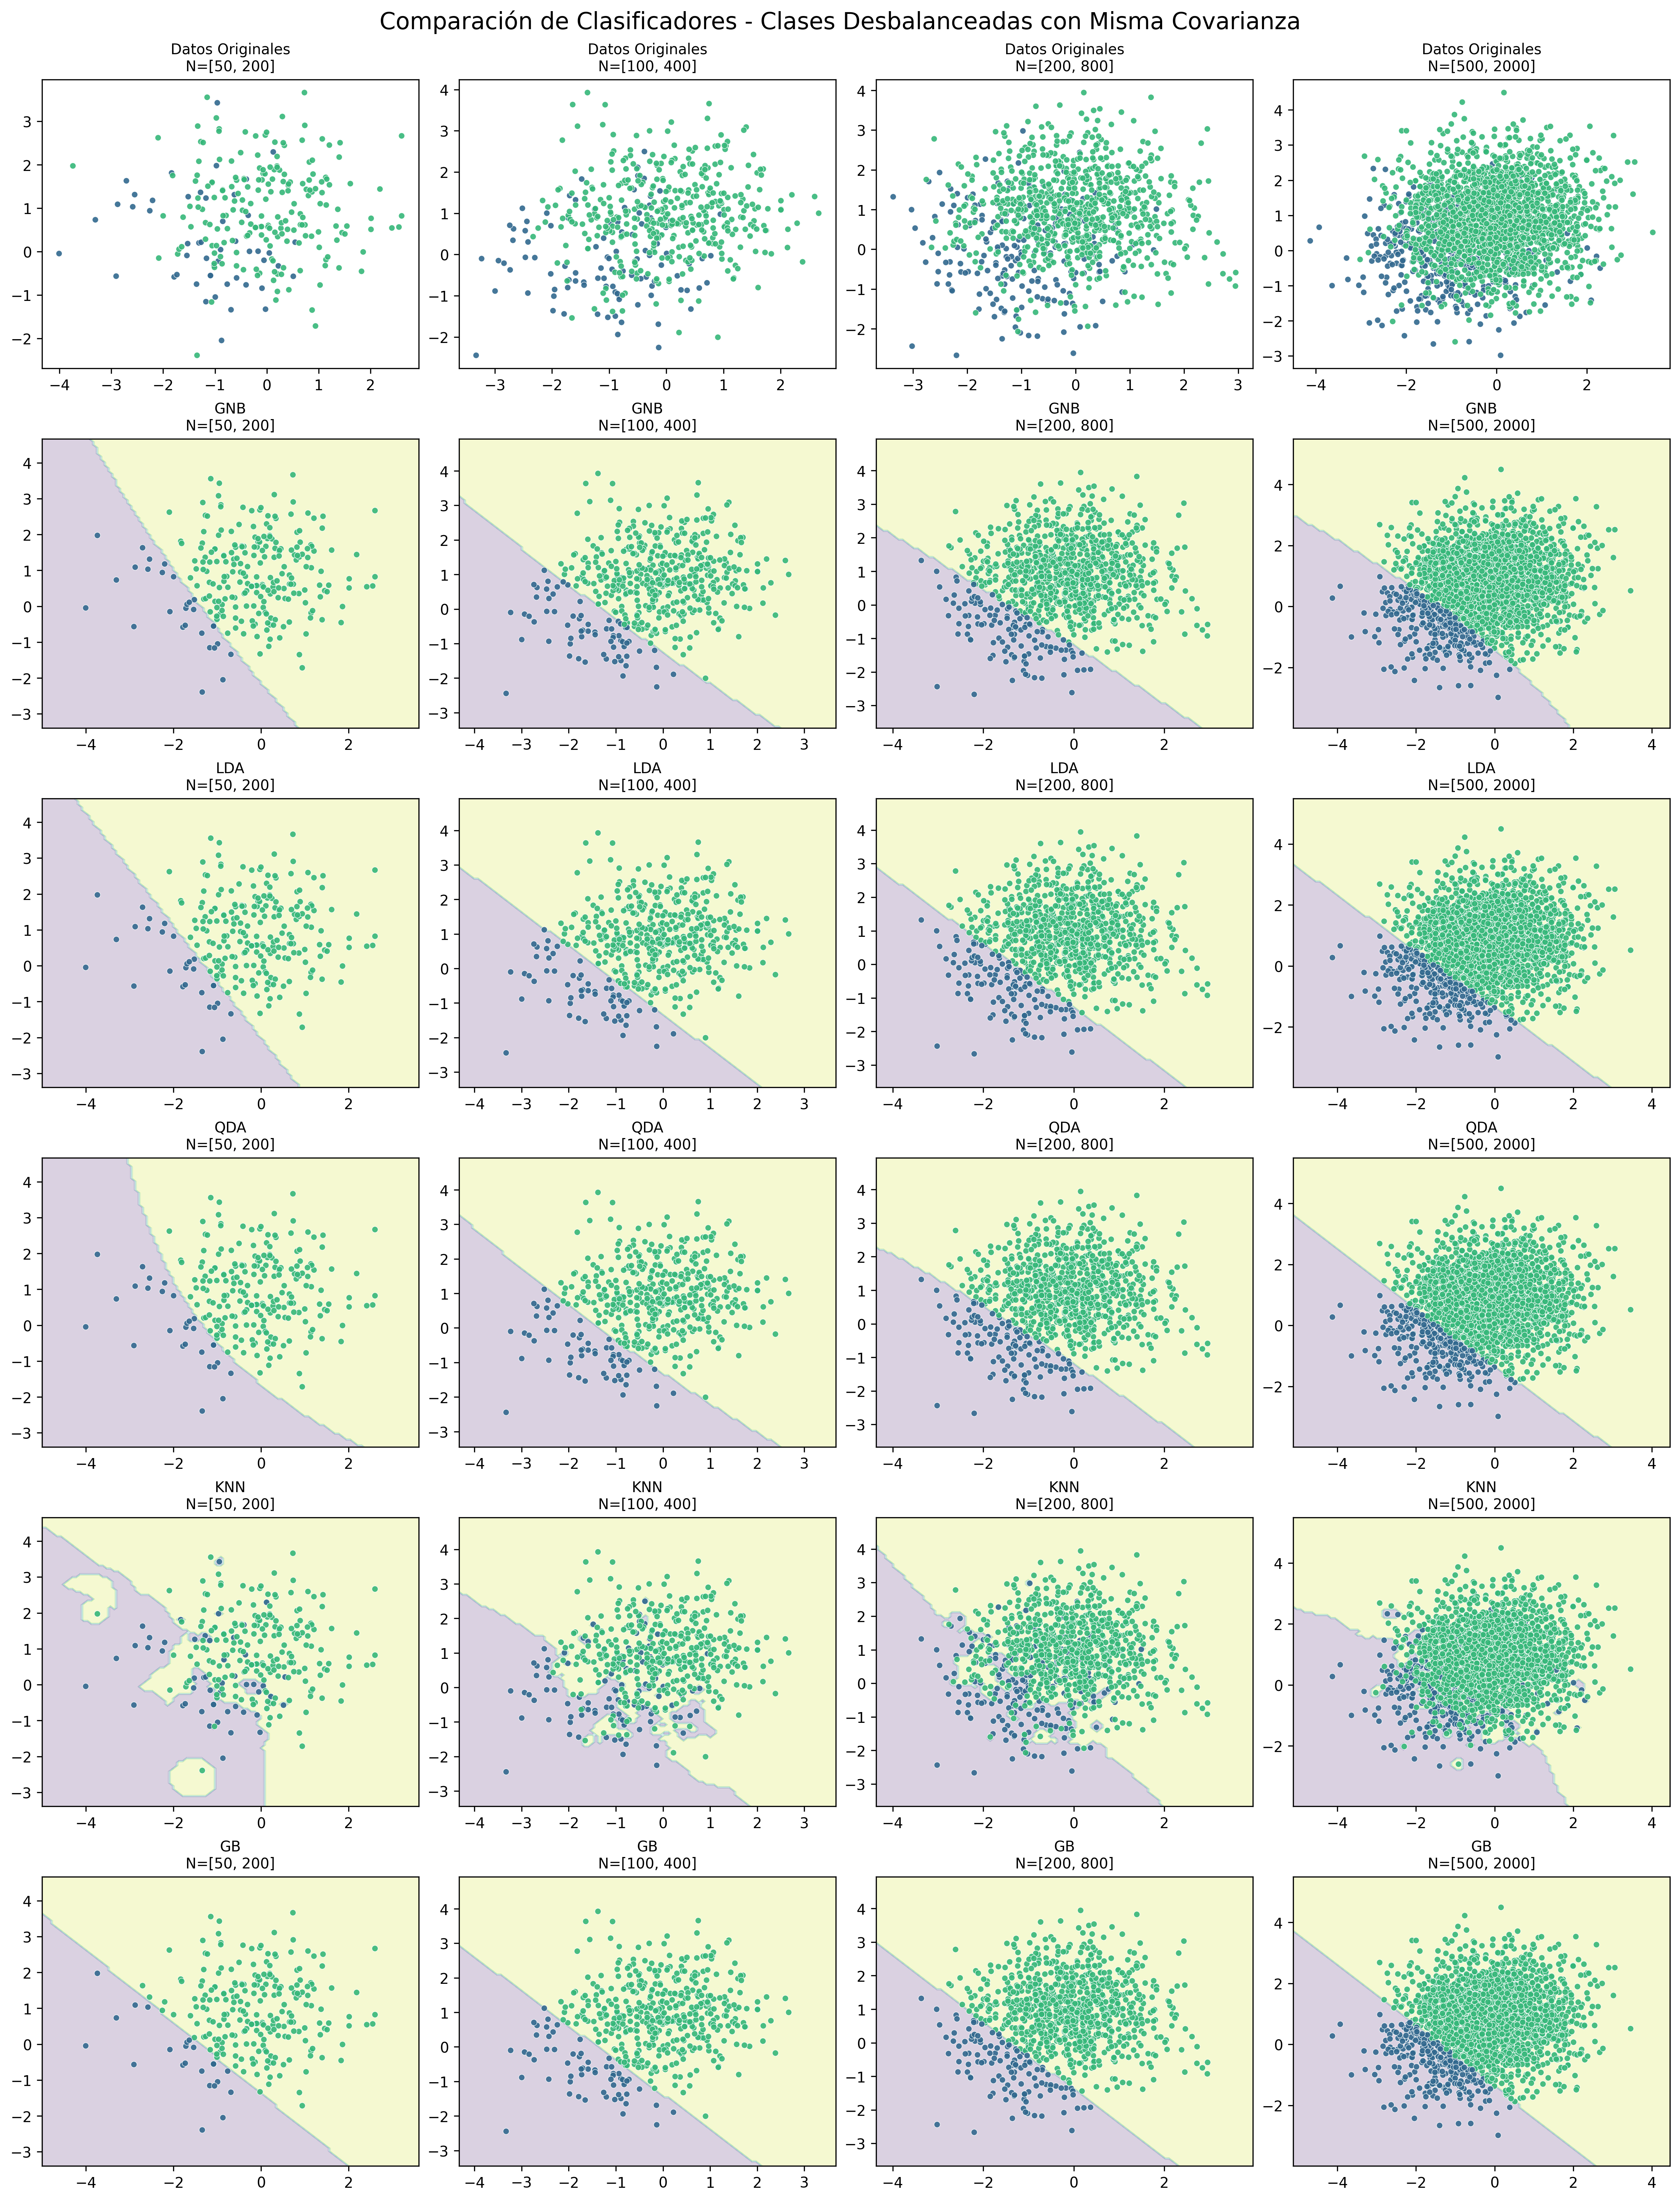
\includegraphics[height=0.4\textheight]{./Parte 2/figures/classifier_comparison_unbalanced_same_cov.png}
    \caption{Comportamiento de clasificadores con datos desbalanceados y covarianzas iguales.}    
    \label{fig:classifier-comparison-unbalanced-same-cov}
\end{figure}

\newpage

Para datos generados con distintas covarianzas se observan las siguientes
comparaciones en la Figura \ref{fig:classifier-comparison-unbalanced-distinct-cov}

\begin{figure}[!ht]
    \centering
    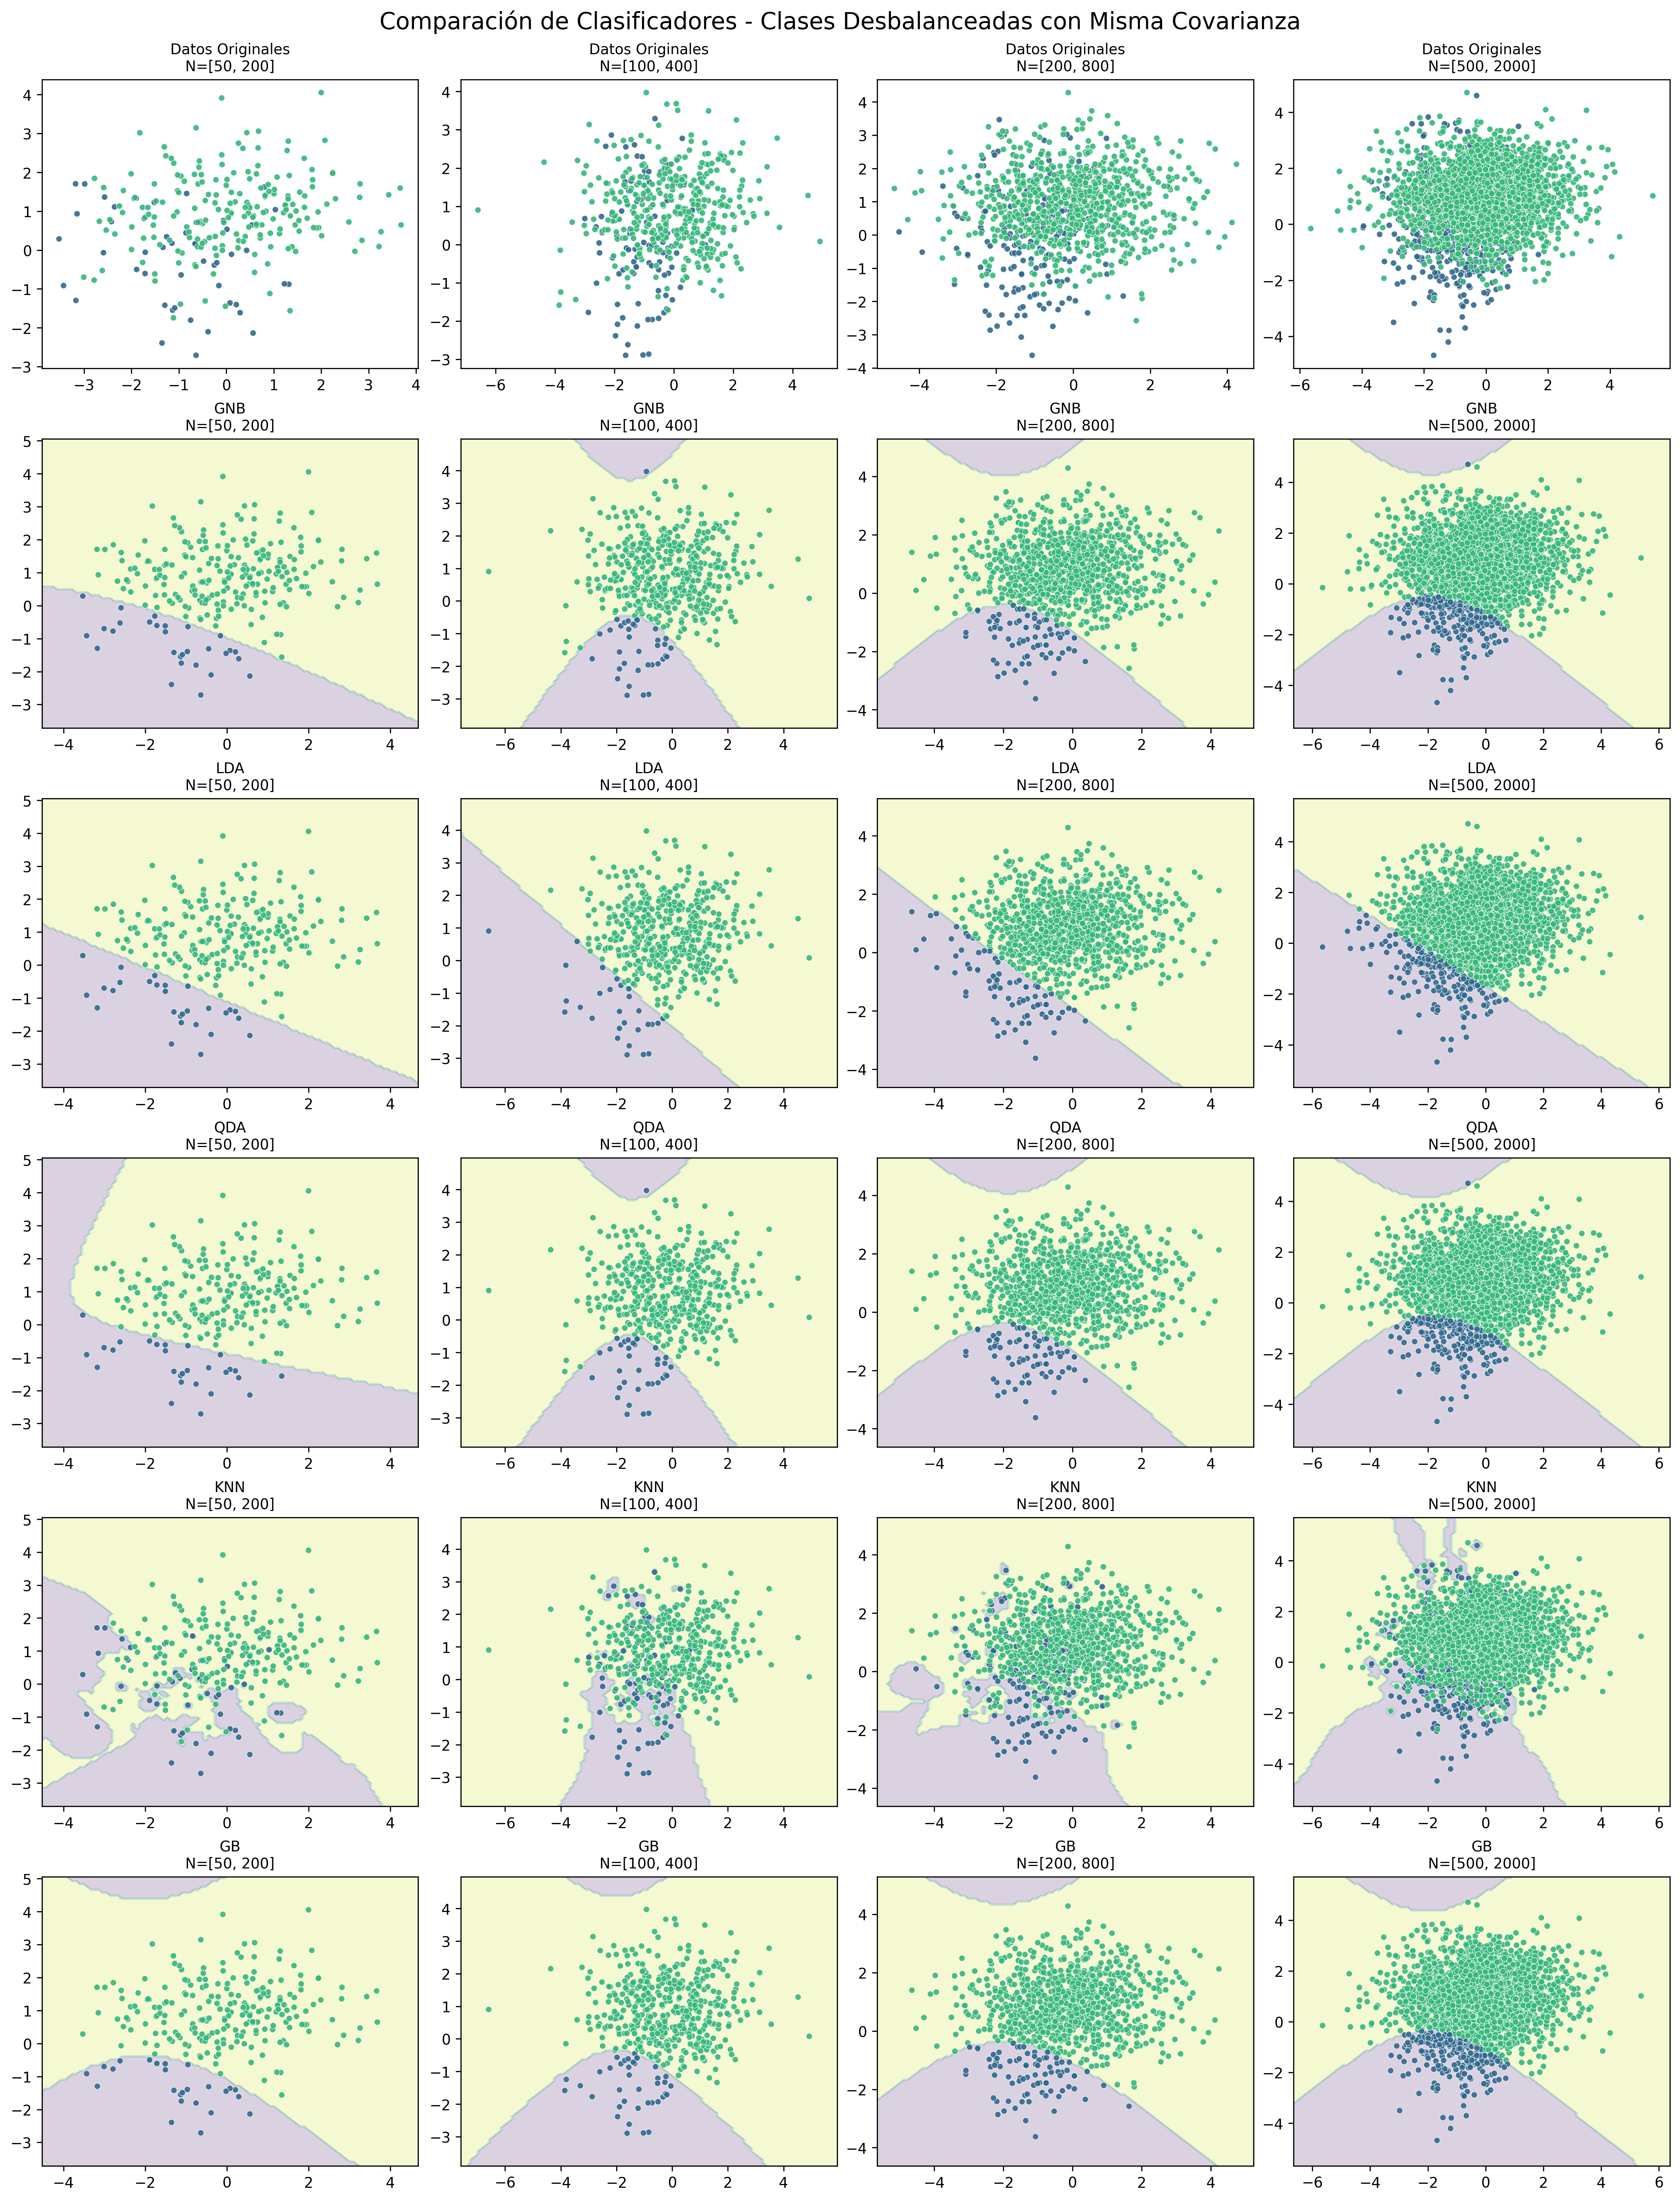
\includegraphics[height=0.4\textheight]{./Parte 2/figures/classifier_comparison_unbalanced_distinct_cov.png}
    \caption{Comportamiento de clasificadores con datos desbalanceados y covarianzas distintas.}    
    \label{fig:classifier-comparison-unbalanced-distinct-cov}
\end{figure}

% Argumentar lo de arriba
\newpage

\subsubsection*{Variando $K$ en \textit{K-NN}}

Ademas, en el algoritmo de \textit{k-NN} se puede variar el valor de $k$ para
obtener diferentes resultados. De mismo modo, consideraremos clases balanceadas
y clases desvalanceadas, ambas con las mismas covarianzas.

Para clases balanceadas se observan las siguientes comparaciones en la Figura
\ref{fig:knn-study-balanced}.

\begin{figure}[!ht]
    \centering
    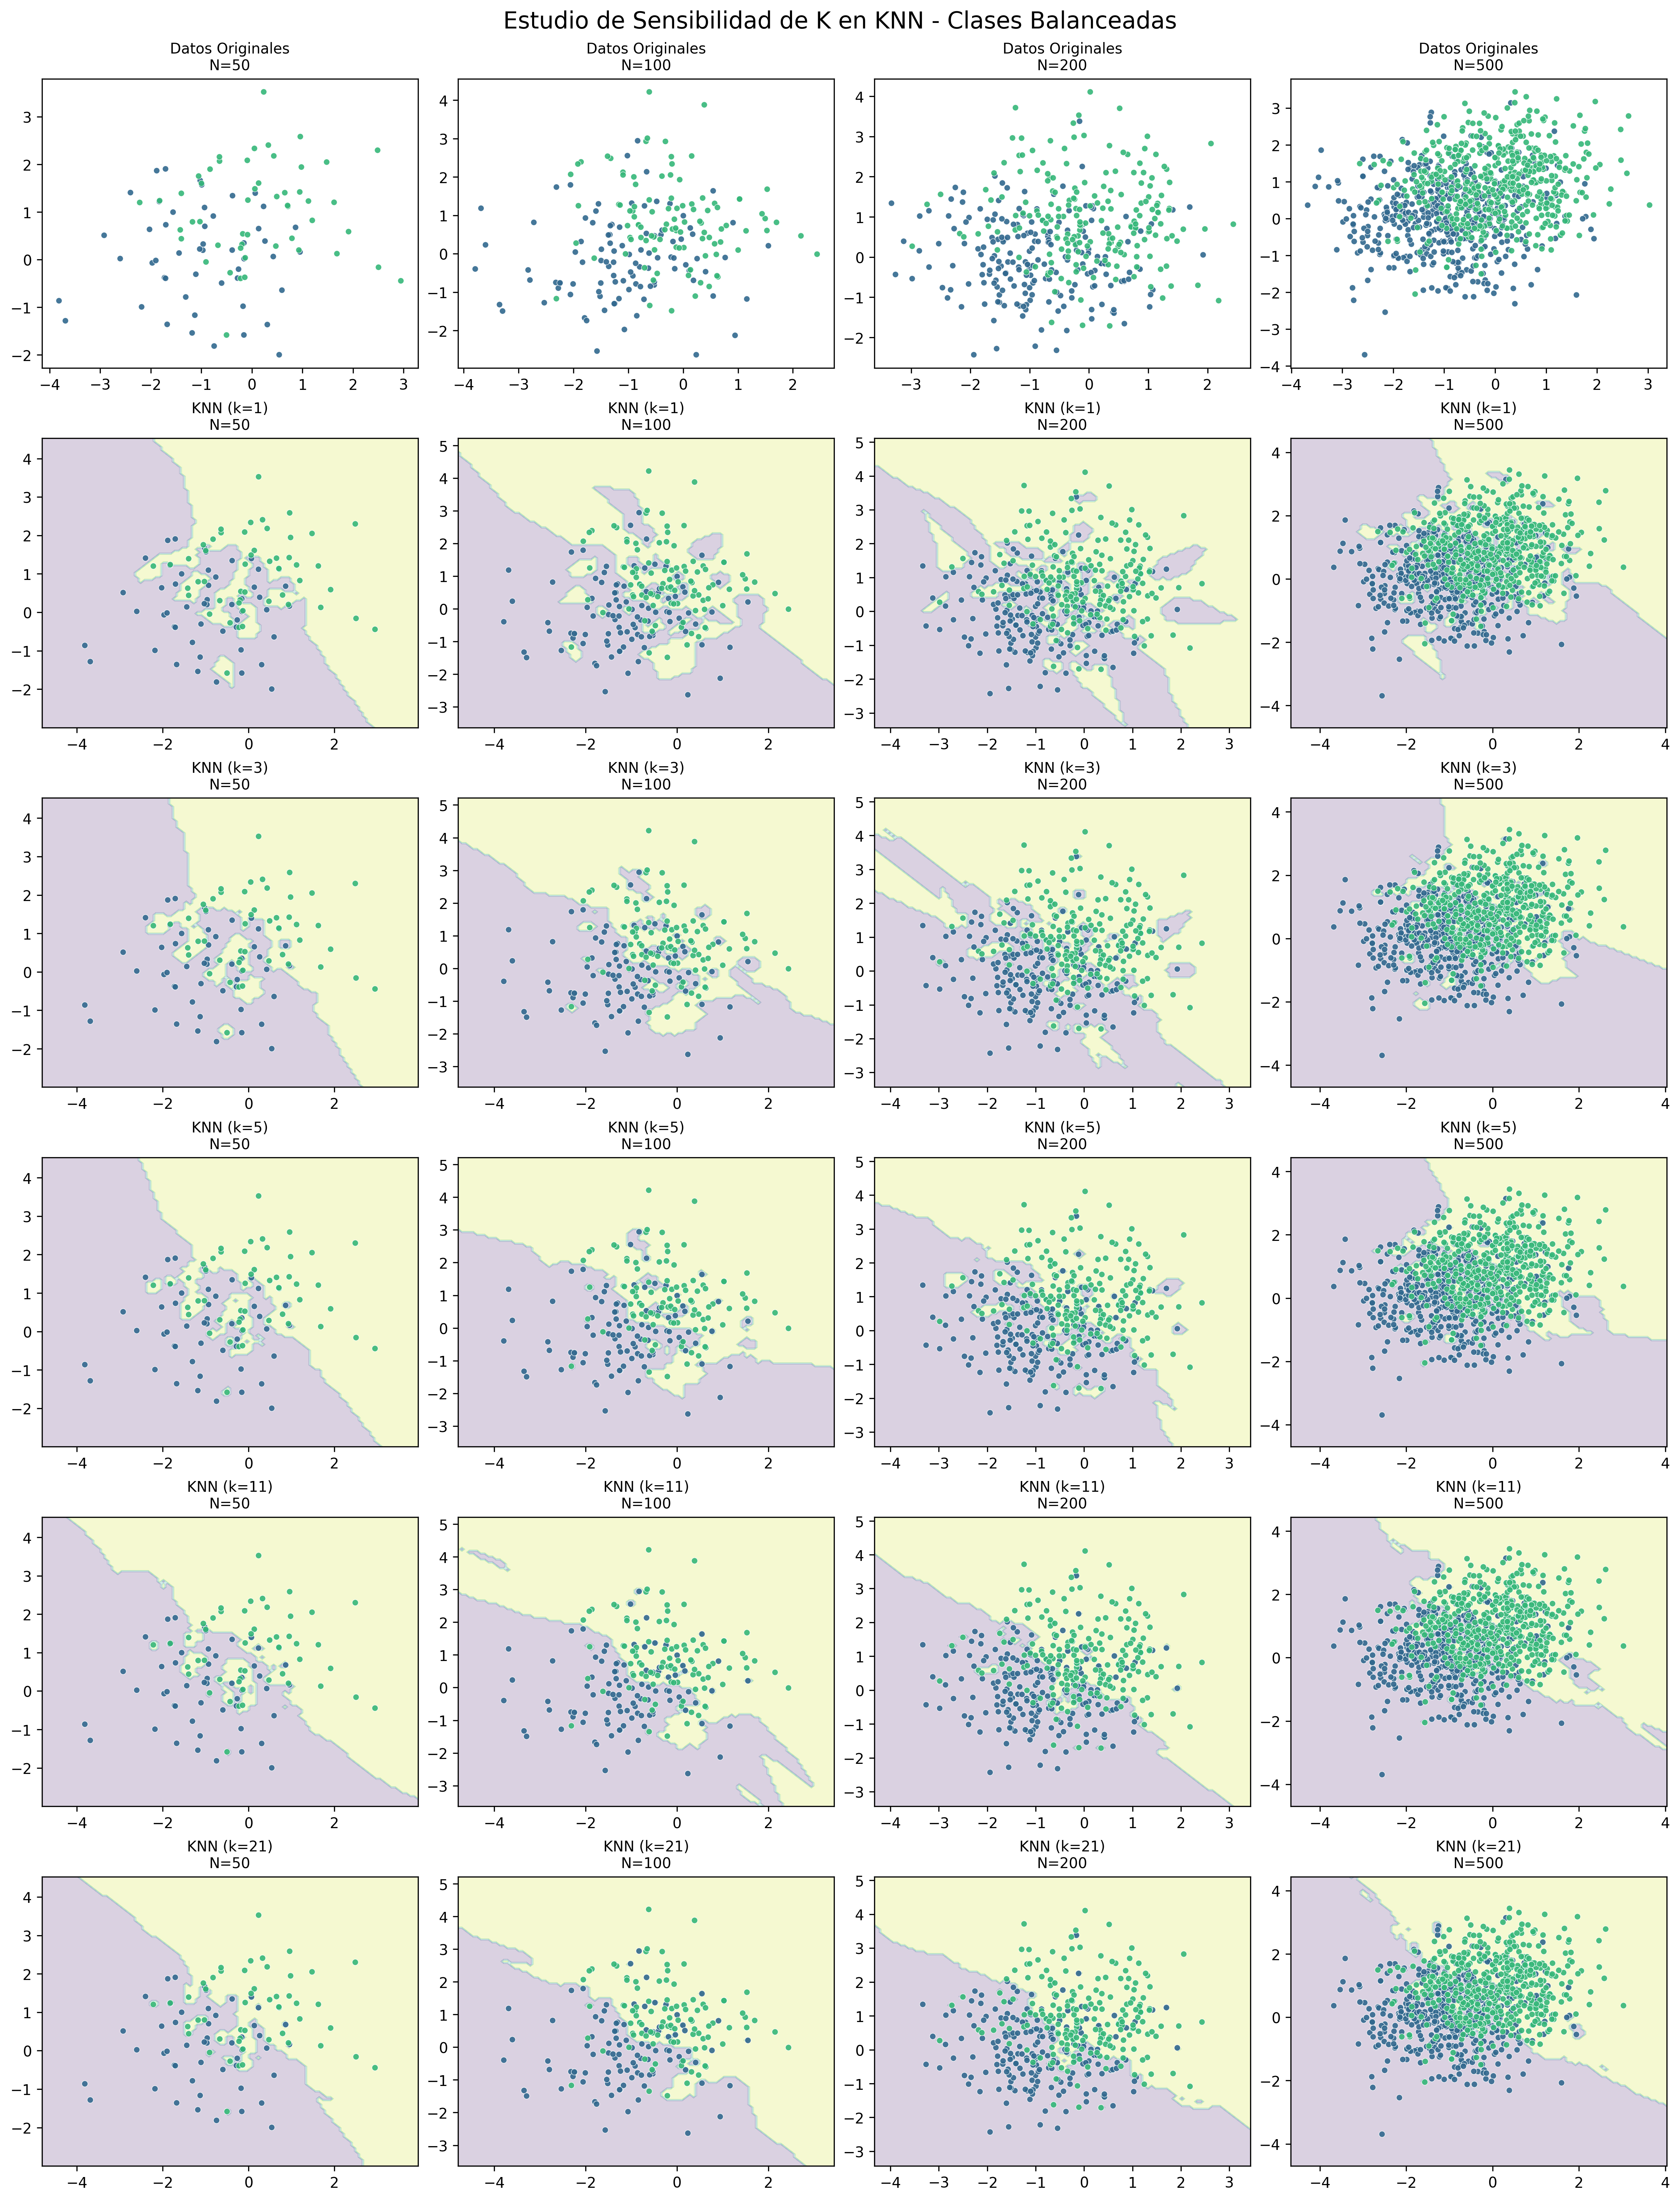
\includegraphics[height=0.4\textheight]{./Parte 2/figures/knn_study_balanced.png}
    \caption{Comportamiento de clasificadores con datos desbalanceados y covarianzas distintas.}    
    \label{fig:knn-study-balanced}
\end{figure}

\newpage

Para clases desbalanceadas se observan las siguientes comparaciones en la Figura
\ref{fig:knn-study-unbalanced}.

\begin{figure}[!ht]
    \centering
    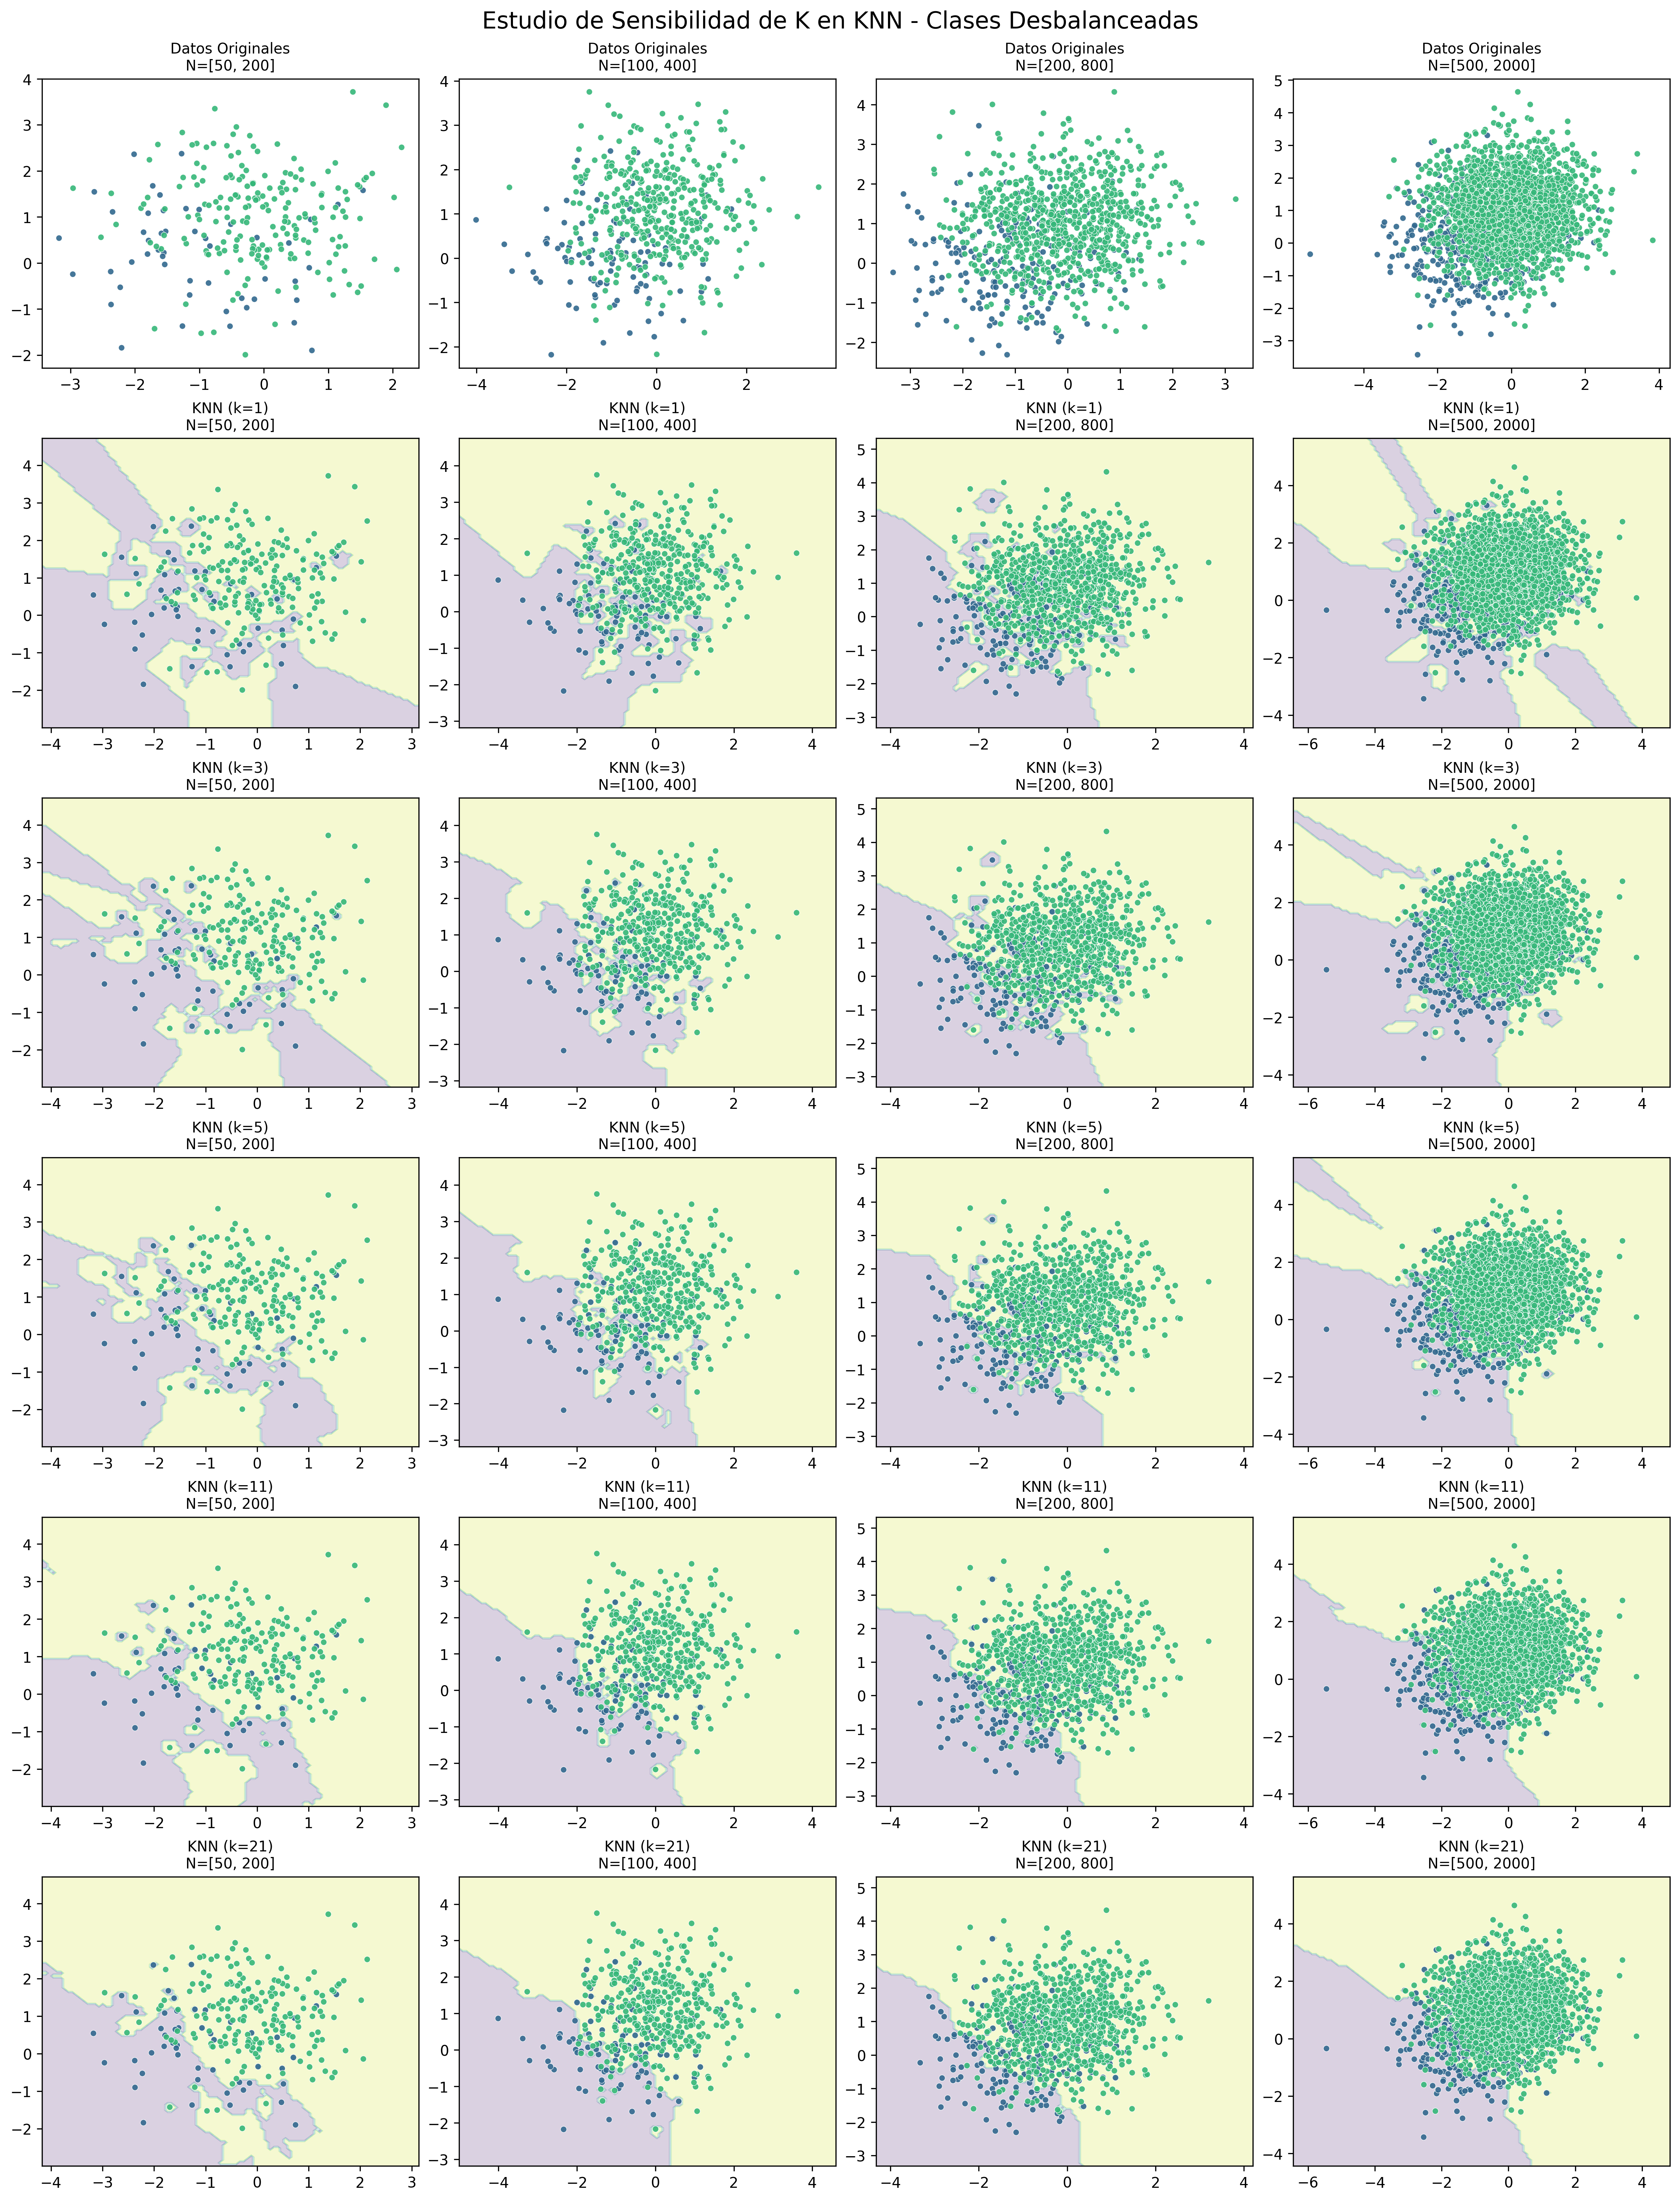
\includegraphics[height=0.4\textheight]{./Parte 2/figures/knn_study_unbalanced.png}
    \caption{Comportamiento de clasificadores con datos desbalanceados y covarianzas distintas.}    
    \label{fig:knn-study-unbalanced}
\end{figure}

% Argumentar lo de arriba
\newpage

\subsection*{Analisis de riesgo}


\begin{figure}[!ht]
    \centering
    \includegraphics[width=0.8\textwidth]{./Parte 2/figures/risk_vs_samplesize.png}
    \caption{}
    \label{fig:risk-vs-samplesize}
\end{figure}

\newpage

\begin{figure}[!ht]
    \centering
    \includegraphics[width=0.4\textwidth]{./Parte 2/figures/risk_gaps.png}
    \includegraphics[width=0.4\textwidth]{./Parte 2/figures/risk_gap_heatmap.png}
    \caption{Risk Gaps $L(g) - L(Bayes)$}
    \label{fig:risk-gaps-images}
\end{figure}

\begin{figure}[!ht]
    \centering
    \includegraphics[width=0.8\textwidth]{./Parte 2/figures/validation_comparison.png}
    \caption{Monte Carlo vs Cross Validation}
    \label{fig:mc-vs-cv}
\end{figure}

\begin{table}[!ht]
    \centering
    \caption{Resumen: Riesgos Promedio y Desviaciones Estándar}
    \label{tab:riesgos_promedio}
    \begin{tabular}{lccc}
        \hline
        \textbf{Modelo} & \textbf{Riesgo Promedio} & \textbf{Desv Estándar} & \textbf{Gap vs Bayes} \\
        \hline
        GaussianNB & 0.2435 & 0.0108 & 0.0037 \\
        LDA & 0.2423 & 0.0103 & 0.0026 \\
        QDA & 0.2441 & 0.0098 & 0.0043 \\
        KNN & 0.2784 & 0.0161 & 0.0386 \\
        \hline
        BAYES & 0.2398 & - & 0 \\
        \hline
    \end{tabular}
\end{table}

\begin{table}[!ht]
    \centering
    \caption{Comparación: Cross-Validation vs Monte Carlo}
    \label{tab:comparacion_cv_mc}
    \begin{tabular}{lcccc}
        \hline
        \textbf{Modelo} & \textbf{CV Risk} & \textbf{CV Std} & \textbf{MC Risk} & \textbf{MC Std} \\
        \hline
        GaussianNB & 0.2460 & 0.0155 & 0.2359 & 0.0049 \\
        LDA & 0.2310 & 0.0284 & 0.2430 & 0.0108 \\
        QDA & 0.2350 & 0.0173 & 0.2351 & 0.0091 \\
        KNN & 0.2920 & 0.0410 & 0.2774 & 0.0128 \\
        \hline
    \end{tabular}
\end{table}

\end{document}